\chapter*{\textcolor{carmillon}{Explication des types choisis}}
Tout d'abord, il a fallu réfléchir à la logique derrière la construction d'un arbre de décision. J'ai réalisé un schéma afin de bien distinguer chaque type, puisque j'ai finalement utilisé deux structures : une structure \textbf{\textit{noeud}} et une structure \textbf{\textit{matrice\_donnees}} qui était fournie. Un schéma des structures est disponible sur la dernière page de ce document.\\

\noindent
La structure \textbf{\textit{matrice\_données}} consiste simplement à rassembler les données d'apprentissage du fichier \textit{iris.txt}. Elle comporte un nombre de lignes, un nombre de colonnes, ainsi qu'une matrice de réels (\textit{double}) qui représente les données d'apprentissage, soit une matrice de 120 lignes et 5 colonnes, les 5 colonnes étant dans l'ordre :\\

\begin{tabular}{|c|c|c|c|c|} 
	\hline
	Espèce de l'iris & Long. sépales & Larg. sépales & Long. pétales & Larg. pétales\\
	\hline
	1, 2 ou 3 & réel & réel & réel & réel\\
	\hline
\end{tabular}\\\\
Avec Setosa $\Leftrightarrow$ 1, Versicolor $\Leftrightarrow$ 2, Virginica $\Leftrightarrow$ 3 pour l'espèce de l'iris.

\noindent
La seconde structure est \textbf{\textit{noeud}} qui représente un noeud de l'arbre. Elle comporte différents attributs :\\

\begin{tabular}{|c|c|c|}
	\hline
	\multicolumn{2}{|c|}{\textbf{Attribut}} & \multirow{2}{2cm}{\textbf{Description}}\\
	\cline{1-2}
	\textbf{Type} & \textbf{Nom} &\\
	\hline
	matrice\_donnees * & donnees & Accès aux données (universel)\\
	\hline
	double & speciesToPredict & Espèce à prédire (Y)\\
	\hline
	int * & listeIndexIndividus & Liste des index des individus de l'échantillon\\
	\hline
	int & tailleEchantillon & Taille de l'échantillon\\
	\hline
	int & xi & Variable de division $X_{i}$ qui a servi à diviser l'éch.\\
	\hline
	double & medCorrected & Médiane corrigée qui a servi à diviser l'éch.\\
	\hline
	char * & critereDivision & Test d'inégalité qui a servi à diviser l'éch. ($\le$ ou $>$)\\
	\hline
	double & precision & Précision de l'éch. par rapport à Y\\
	\hline
	struct \_noeud & parent & Noeud parent du noeud actuel\\
	\hline
	struct \_noeud & fils\_gauche & Fils gauche du noeud actuel\\
	\hline
	struct \_noeud & fils\_droite & Fils droit du noeud actuel\\
	\hline
\end{tabular}\\\\

\chapter*{\textcolor{carmillon}{Explication de la création de l'arbre}}

Premièrement, on charge notre fichier texte dans notre structure \textbf{\textit{matrice\_donnees}}, et on initialise notre racine avec l'intégralité de notre échantillon à l'aide de la fonction \textbf{\textit{initialiser\_racine}}.
Par la suite, pour créer l'arbre de décision, on regarde d'abord si notre échantillon peut être divisé, à l'aide de la fonction \textbf{\textit{canBeDivided}}. S'il ne peut pas, alors on ne fait rien (condition d'arrêt). Sinon, on récupère d'abord le meilleur critère de division à l'aide de la fonction \textbf{\textit{bestDivision}}. Ce critère correspond au $X_{i}$ à utiliser pour diviser l'échantillon (1, 2, 3 ou 4). On crée ensuite le tableau des valeurs triées pour l'échantillon avec \textbf{\textit{triSelonX}}. Ce tableau sera utilisé pour calculer la médiane et la médiane corrigée de l'échantillon. On calcule maintenant d'abord la médiane, puis la médiane corrigée. On crée 2 tableaux d'entiers, qui sont nos sous échantillons respectifs (gauche et droite), c'est à dire la liste des individus dont la valeur de $X_{i}$ est $\le$ ou > à la médiane corrigée. On calcule également la taille de ces sous échantillons.
On crée 2 noeuds (les fils gauche et droit) à qui on affecte leur liste d'individus et leur taille d'échantillon. On leur affecte également leur critère de division ($X_{i}$, médiane corrigée et test d'inégalité) ainsi que leur précision.
Pour finir, on affecte les fils gauche et droit au noeud actuel, et on associe le noeud actuel comme parent des fils. On rappelle récursivement la fonction avec les fils gauche et droit, en n'oubliant pas de changer le paramètre \textbf{\textit{hauteurMax}} à \textbf{\textit{hauteurMax - 1}} car on descend d'un cran dans la génération, donc la hauteur de l'arbre augmente consécutivement.

\chapter*{\textcolor{carmillon}{Descriptif des fonctions}}
\textbf{1. Hauteur de l'arbre :} La fonction hauteurArbre prend un \textbf{\textit{noeud}} en paramètre. Elle regarde si elle possède un fils gauche et un fils droit. Si oui, on rappelle récursivement la fonction sur le fils concerné, et lorsque le parcours est terminé (plus de descendants), on retourne simplement 1 (noeud actuel) + la profondeur maximum entre les deux fils (trouvée à l'aide d'une petite fonction qui calcule le maximum entre deux entiers).\\

\noindent
\textbf{2. Largeur de l'arbre :} La fonction largeurArbre prend un \textbf{\textit{noeud}} en paramètre. Si il est NULL, alors on retourne 0, sinon : on regarde si c'est une feuille (ie. si ses fils sont NULL). Si c'est le cas, on retourne 1, sinon on appelle récursivement la fonction pour les deux fils.\\

\noindent
\textbf{3. Affichage en arborescence :} La fonction affichageArborescence prend un \textbf{\textit{noeud}} en paramètre. Si le noeud n'est pas NULL, tout d'abord on affiche l'offset (lorsque le noeud n'est pas racine, l'offset est > 0) puis son contenu (ie. le $X_{i}$, le test d'inégalité, la médiane corrigée, la taille de l'échantillon et sa précision). On appelle ensuite récursivement affichageArborescence pour les fils gauche et droit, en modifiant le paramètre \textbf{\textit{offset}} à \textbf{\textit{offset + 1}} car on descend d'un cran dans les générations. Lors de l'appel initial de la fonction, offset vaut 0.\\

\noindent
\textbf{4. Afficher les feuilles :} La fonction afficherFeuilles prend un \textbf{\textit{noeud}} en paramètre. S'il n'est pas NULL, alors on regarde si c'est une feuille (ie. si ses fils sont NULL). Si c'est le cas, on affiche le noeud (son $X_{i}$, son test d'inégalité et sa médiane corrigée), ainsi que son chemin à l'aide de la fonction \textbf{\textit{afficherChemin}}. Sinon, on appelle récursivement la fonction pour les deux fils.\\

\noindent
\textbf{5. Prédire :} La fonction prédire prend un \textbf{\textit{noeud}} et 4 valeurs de $X_{i}$ en paramètre. Si le noeud actuel est une feuille (ie. on est arrivé au bout de l'arbre avec les valeurs données de $X_{i}$, soit condition d'arrêt), alors on retourne la précision du noeud. Sinon, on trouve la direction que l'on doit prendre pour le noeud suivant en fonction du $X_{i}$ du noeud, de sa médiane corrigée et de notre $X_{i}$ correspondant ($X_{i}\le$Med $\Leftrightarrow$ A gauche, $X_{i}$>Med $\Leftrightarrow$ A droite). On rappelle ensuite notre fonction prédire avec comme paramètre les mêmes valeurs de $X_{i}$ et le fils gauche ou droit selon la direction que l'on a du prendre. \\

\begin{tabular}{|c|c|c|c|c|c|} 
	\cline{2-6}  
	\multicolumn{1}{c|}{} & Précision pour Y = 2 & $\displaystyle{X_{1}}$ & $\displaystyle{X_{2}}$ & $\displaystyle{X_{3}}$ & $\displaystyle{X_{4}}$\\
	\hline
	1 & 3.44828\% & 7.7 & 3.0 & 6.1 & 2.3\\
	\hline
	2 & 3.44828\% & 6.2 & 2.8 & 4.8 & 1.8\\
	\hline
	3 & 100\% & 5.5 & 2.5 & 4.0 & 1.3\\
	\hline
	4 & 0\% & 6.7 & 3.3 & 5.7 & 2.5\\
	\hline
	5 & 94.4444\% & 6.0 & 2.2 & 5.0 & 1.5\\
	\hline
	6 & 3.44828\% & 6.0 & 2.7 & 5.1 & 1.6\\
	\hline
	7 & 100\% & 5.7 & 2.6 & 3.5 & 1.0\\
	\hline
	8 & 100\% & 5.8 & 2.6 & 4.0 & 1.2\\
	\hline
	9 & 0\% & 5.1 & 3.4 & 1.5 & 0.2\\
	\hline
	10 & 0\% & 5.4 & 3.9 & 1.3 & 0.4\\
	\hline
\end{tabular}

\begin{figure}[H]
	\begin{center}
		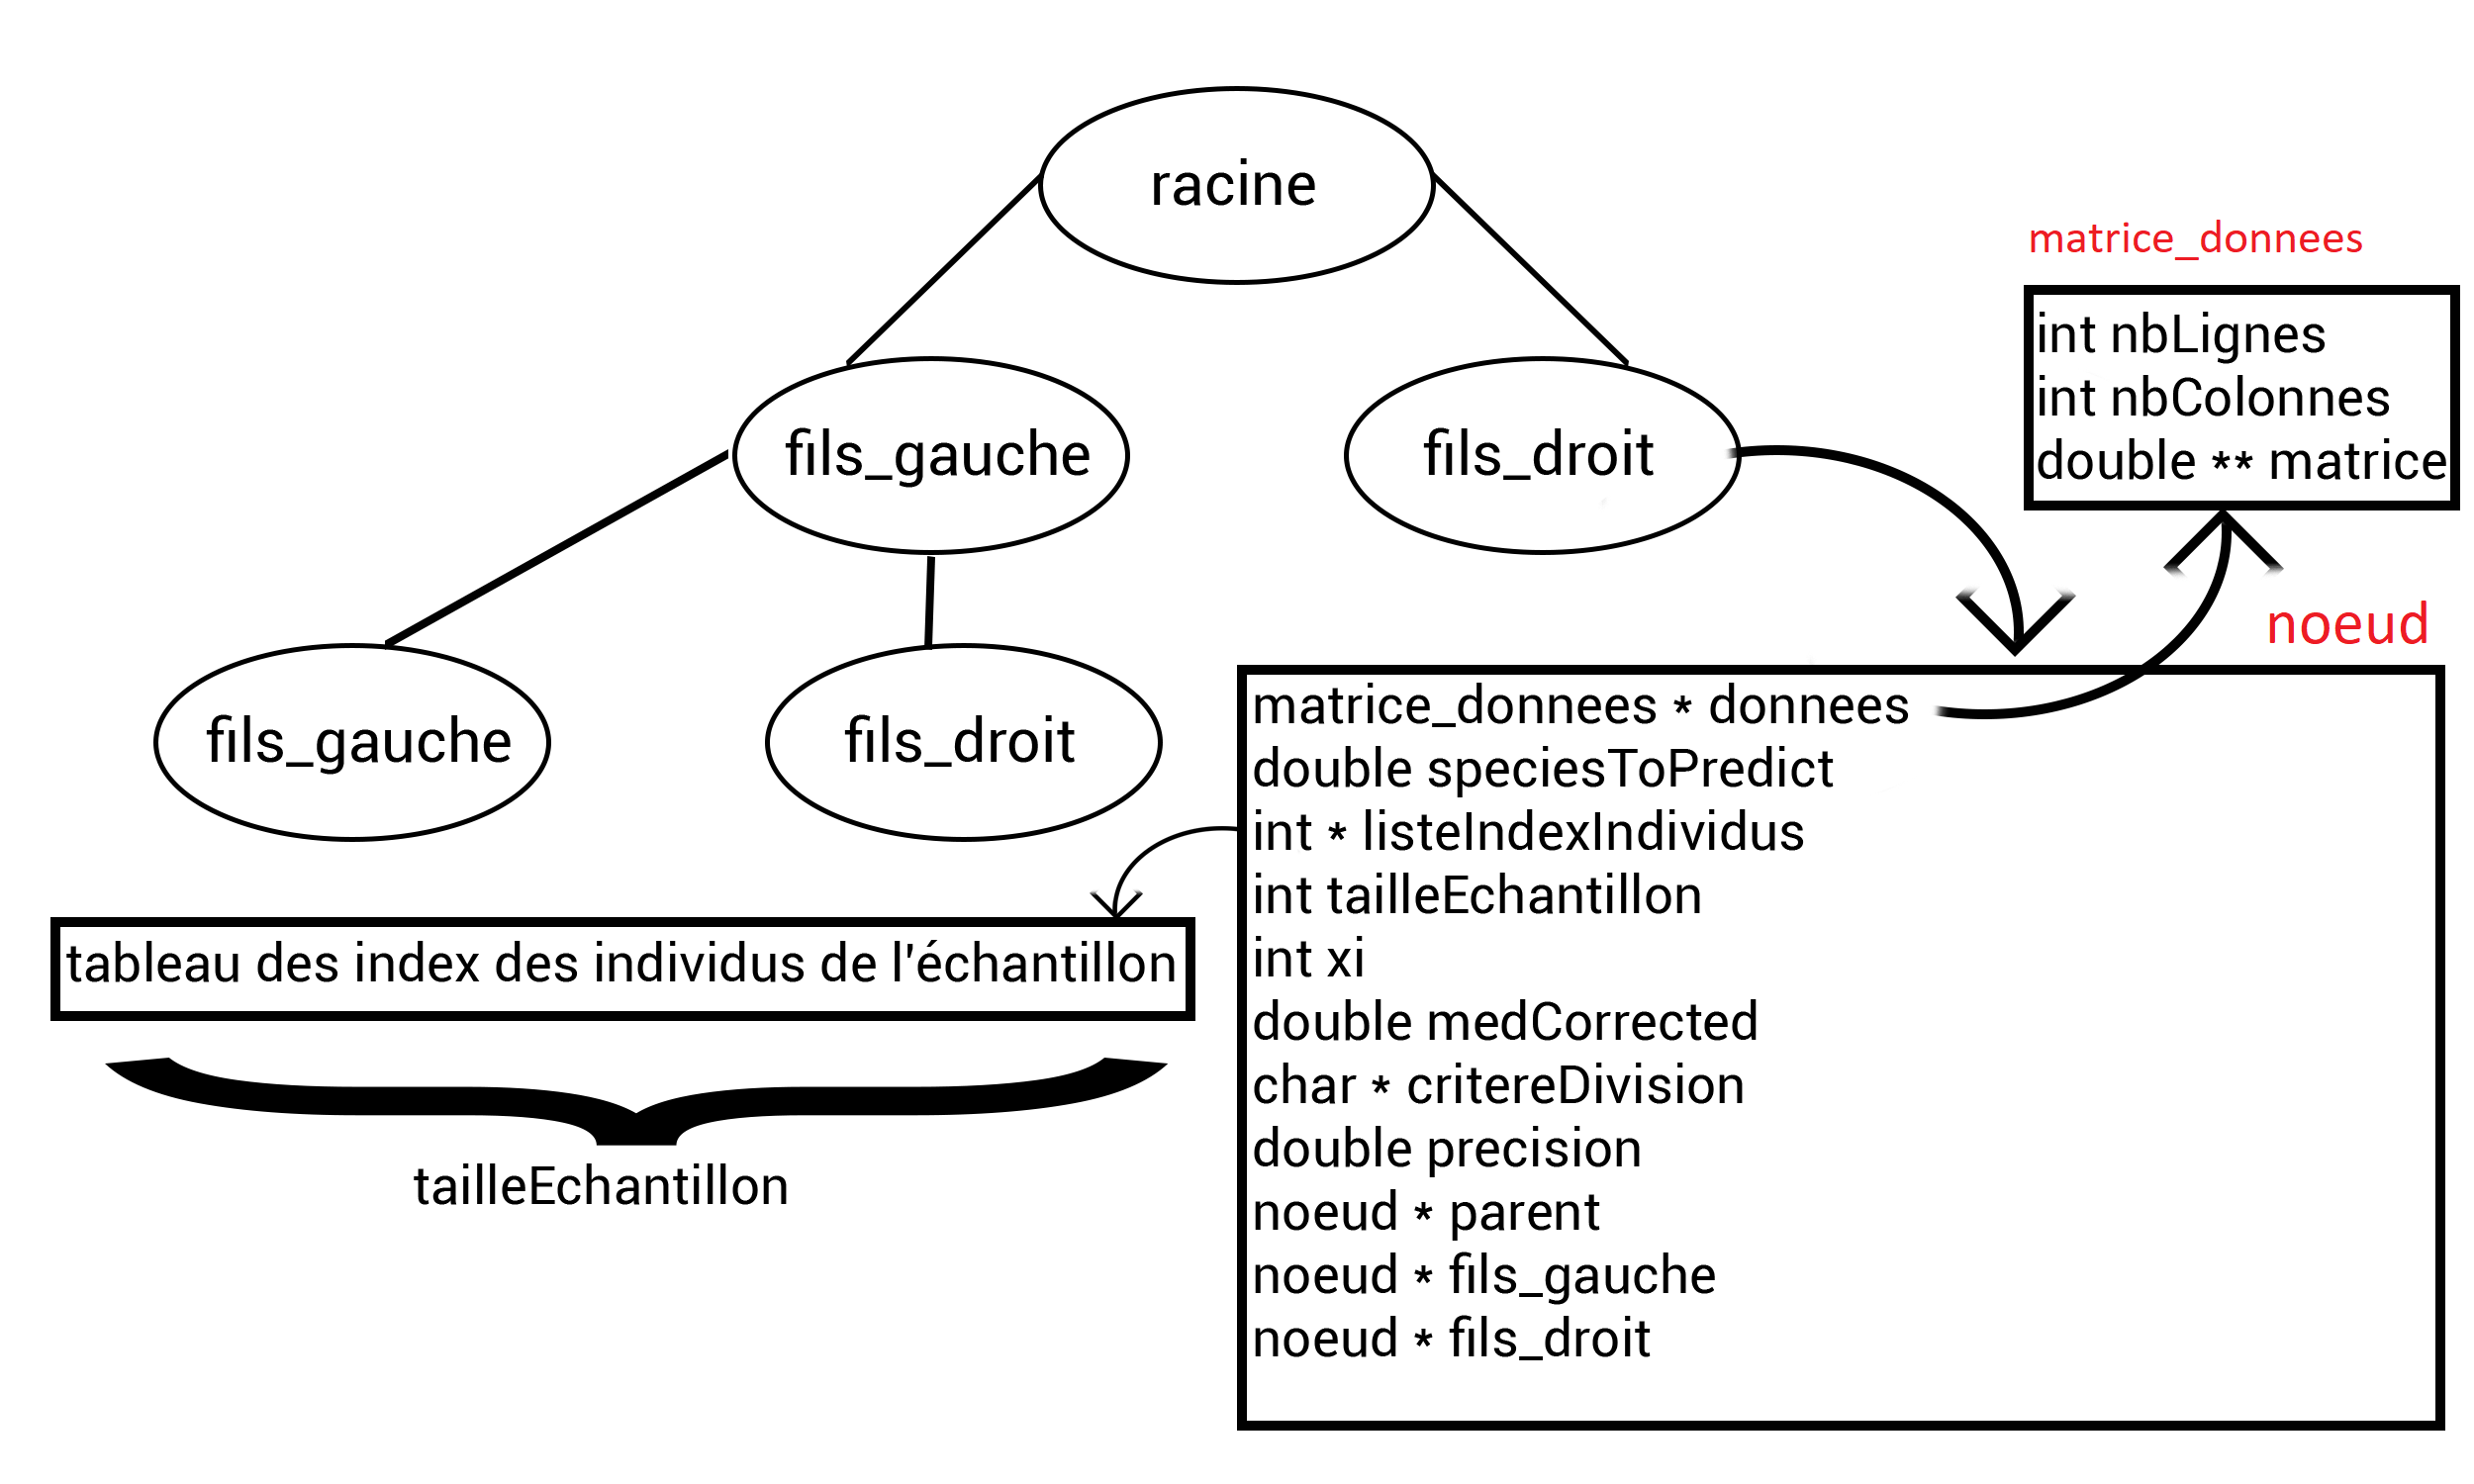
\includegraphics[scale=0.27]{./img/schema.png}
	\end{center}
	\caption{Organisation des structures}
\end{figure}